\documentclass{article}

% Esto es para poder escribir acentos directamente:
\usepackage[utf8]{inputenc}
% Esto es para que el LaTeX sepa que el texto est en espaol:
\usepackage[spanish, activeacute]{babel}

% Paquetes de la AMS:
\usepackage{amsmath, amsthm, amsfonts}

\usepackage{graphicx}
\graphicspath{ {images/} }

\usepackage[margin=1in]{geometry}

\usepackage{listings}

% Teoremas
%--------------------------------------------------------------------------
\newtheorem{thm}{Teorema}[section]
\newtheorem{cor}[thm]{Corolario}
\newtheorem{lem}[thm]{Lema}
\newtheorem{prop}[thm]{Proposicin}
\theoremstyle{definition}
\newtheorem{defn}[thm]{Definicin}
\theoremstyle{remark}
\newtheorem{rem}[thm]{Observacin}

% Atajos.
% Se pueden definir comandos nuevos para acortar cosas que se usan
% frecuentemente. Como ejemplo, aqu se definen la R y la Z dobles que
% suelen representar a los conjuntos de nmeros reales y enteros.
%--------------------------------------------------------------------------

\def\RR{\mathbb{R}}
\def\ZZ{\mathbb{Z}}

% De la misma forma se pueden definir comandos con argumentos. Por
% ejemplo, aqu definimos un comando para escribir el valor absoluto
% de algo ms fcilmente.
%--------------------------------------------------------------------------
\newcommand{\abs}[1]{\left\vert#1\right\vert}

% Operadores.
% Los operadores nuevos deben definirse como tales para que aparezcan
% correctamente. Como ejemplo definimos en jacobiano:
%--------------------------------------------------------------------------
\DeclareMathOperator{\Jac}{Jac}

\lstset{morecomment=[l][\color{Green}]{\#\ },numbers=left,numberstyle=\tiny,frame=tLBr,%
emph={function, while, end, if, for},emphstyle=\color{Blue},escapeinside=||}

%--------------------------------------------------------------------------
\title{Nuevas Tecnologías de la Programación \\ Práctica 3}
\author{Javier Moreno}

\begin{document}
\maketitle

\abstract{Informe de la práctica 3 de la asignatura Nuevas tecnologías de la programación.}

\section{Introducción}


\newpage
\section{Diseño}
\subsection{Diagrama de clases}
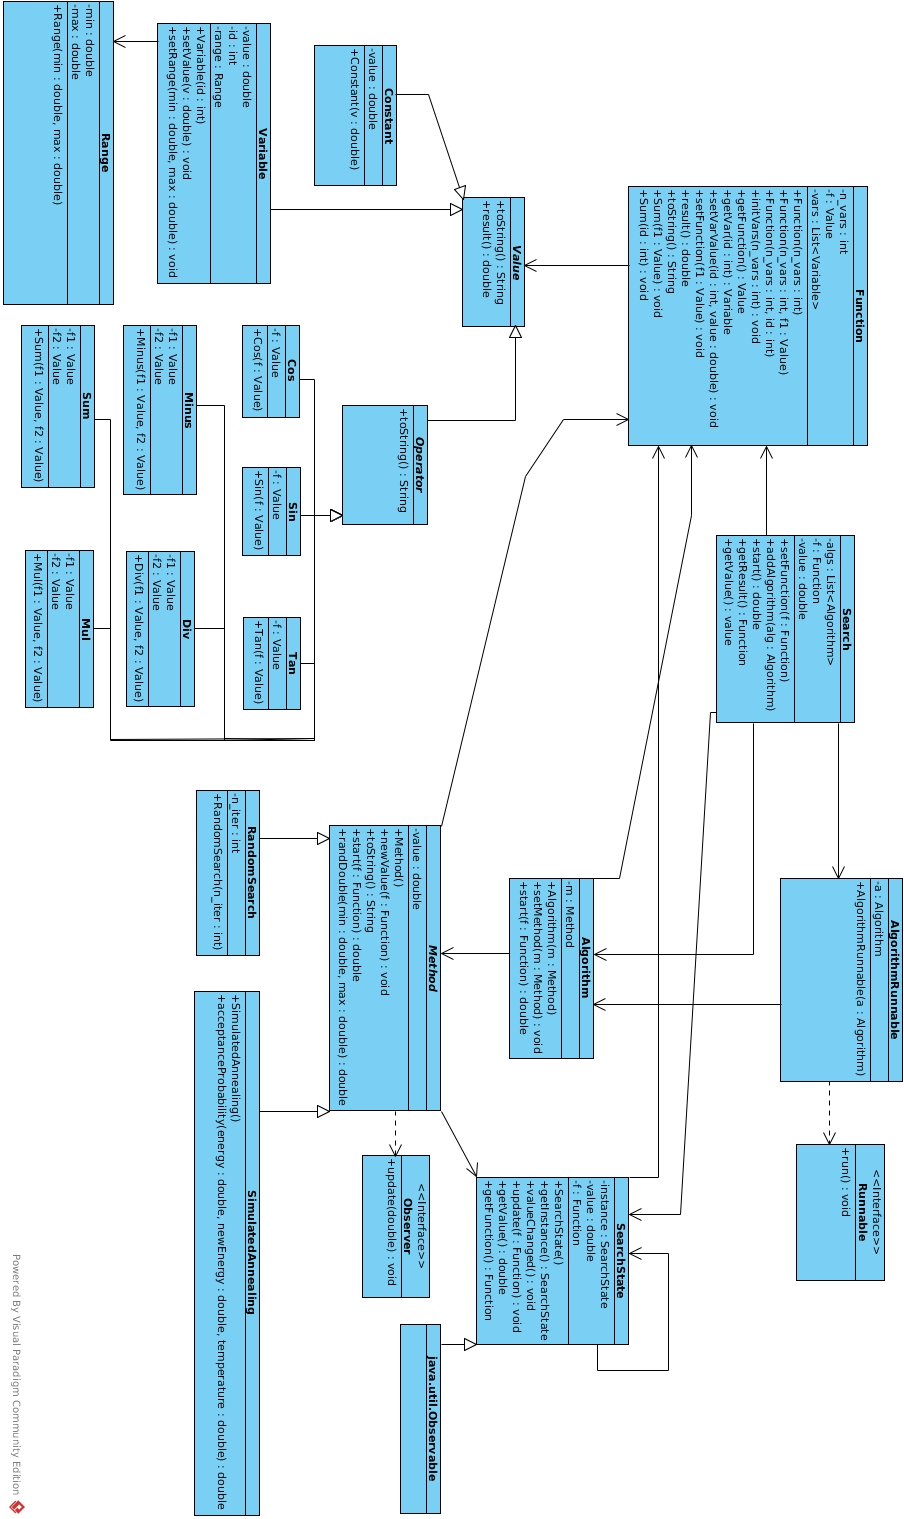
\includegraphics[scale=0.4]{diagram.jpg}
\subsection{Explicación}
Patrones usados
Clases definidas

\newpage
\section{Ejemplo de uso}
\begin{lstlisting}[language=Java]
// Objeto f de la clase Function que contendra la funcion a optimizar.
Function f = new Function(2);

// Se definen las operaciones, constantes y variables de la funcion.
f.Sin(new Mul(new Mul(new Constant(20), new Constant(3.14)), f.getVar(1)));
f.Mul(1);
f.Sum(new Mul(f.getVar(0), new Sin(new Mul(new Mul(new Constant(4), 
	new Constant(3.14)), f.getVar(0)))));
f.Sum(new Constant(21.5));
        
// Rango de las variables.
f.getVar(0).setRange(-3, 12.1);
f.getVar(1).setRange(4.1, 5.8);
        
// Objeto e de la clase Search que controla la busqueda de valores maximos.
Search e = new Search();
// Se anade la funcion a optimizar.
e.setFunction(f);
// Se anaden los algoritmos de busqueda que se quieran usar.
e.addAlgorithm(new Algorithm(new RandomSearch(10000)));
e.addAlgorithm(new Algorithm(new SimulatedAnnealing()));
// Inicio de la busqueda.
e.start();
        
// Se escribe por pantalla la funcion a optimizar.
System.out.println("f()="+f.toString());
// Se escribe por pantalla el mejor valor encontrado.
System.out.println("Best Value: "+e.getValue());
\end{lstlisting}
\end{document}






